\chapter{Arquitectura de la solución}\label{arquitectura}
El ECG (Electrocardiograma) detecta señales del cuerpo gracias a electrodos que se colocan en la superficie del cuerpo, usualmente acompañados de un gel conductor que elimina interferencia de los músculos, fuente de alimentación,  ruido externo, etc. Para que se obtenga una señal de ECG sin distorsiones excesivas, es necesario diseñar filtros que eliminen interferencias antes de analizar la información. \\

\section{DFRobot Heart Rate Monitor}\label{reqfuncional1asc}
El monitor de actividad cardíaca de la empresa DFRobot consiste en una placa que consta de un chip AD8232 en su PCB, el cual provee una clara señal de los intervalos PR y QT (Ver Figura \ref{onda})  de un electrocardiograma. Este entrega un valor análogo que puede ser leído por Arduino y con un conversor análogo-digital interpretarse en forma de gráfico.\\

\begin{figure}[H]
\centering
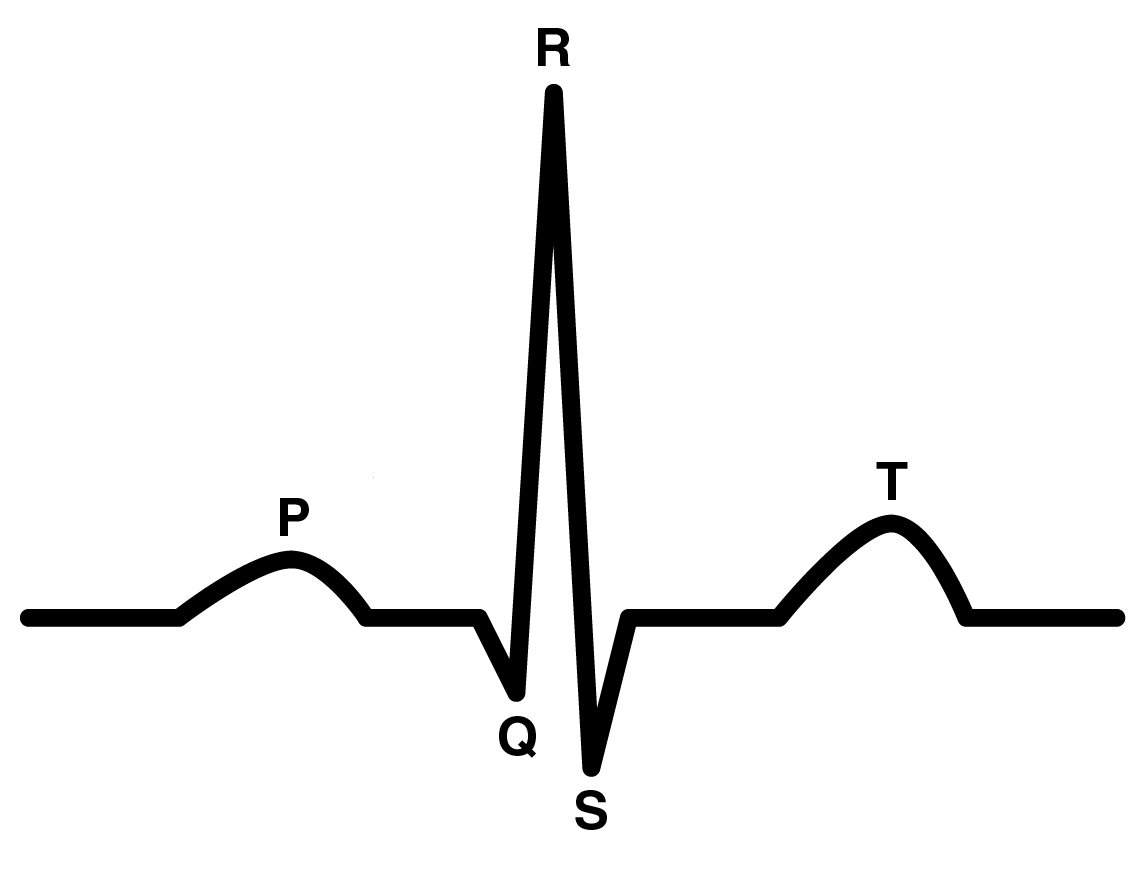
\includegraphics[scale=0.2]{figuras/ecg/senal.png}
\caption{Forma de onda teórica ECG}
\label{onda}
\end{figure}

Se escogió esta placa de desarrollo por disponibilidad de hardware, ya que es la única opción disponible de bajo costo, y que no necesita comprarse fuera del país. Por lo que se tomó la decisión de estudiar su funcionamiento, replicarlo para el diseño del dispositivo final y evaluar posibles mejoras. \\

\section{Biopac MP150 ECG100C}
Se tuvo la oportunidad de usar el ECG de la empresa Biopac ECG100C, el cual es de mucho mayor costo y tamaño utilizado generalmente para investigación. La idea era ver la forma de onda y comparar las frecuencias de corte utilizadas. La figura \ref{biopac} muestra el aparato encargado de tomar las señales de los electrodos y la figura \ref{frecuencias} muestra un acercamiento con las posibles frecuencias de corte configurables para los filtros.\\

\begin{figure}[H]
\centering
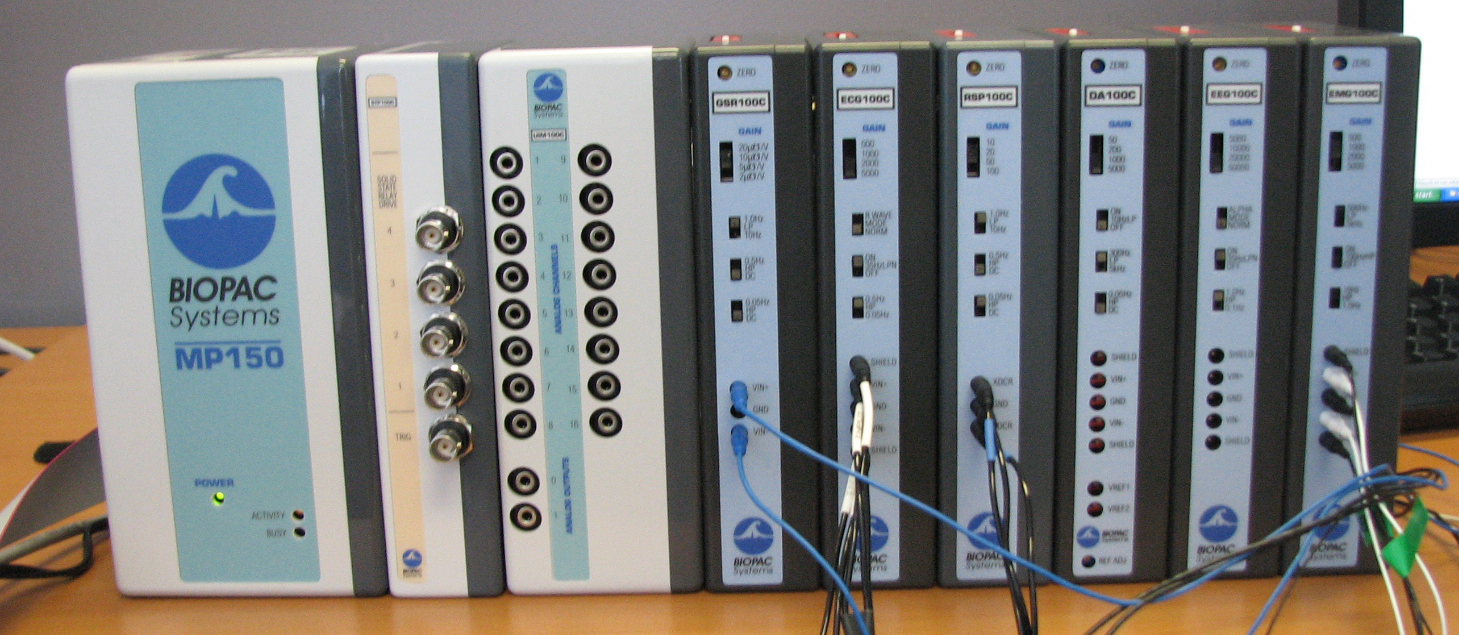
\includegraphics[scale=0.7]{figuras/ecg/biopac.jpg}
\caption{Biopac MP150}
\label{biopac}
\end{figure}

\begin{figure}[H]
\centering
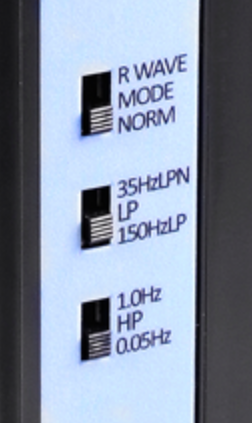
\includegraphics[scale=0.7]{figuras/ecg/biopacecg.png}
\caption{Frecuencias de corte disponibles en Biopac ECG100C}
\label{frecuencias}
\end{figure}

Cabe destacar el alto precio de este equipo que es de 45.000 USD y grandes dimensiones ya que está diseñado para investigación lo cual servirá para saber donde tiene que apuntar la forma de onda de un ECG de grado médico.\\

\newpage
\section{AD8232}
El chip AD8232 es un integrado que permite medir las señales de los electrodos del ECG mediante amplificadores operacionales como se muestra en la figura \ref{ad8232}.

\begin{figure}[H]
\centering
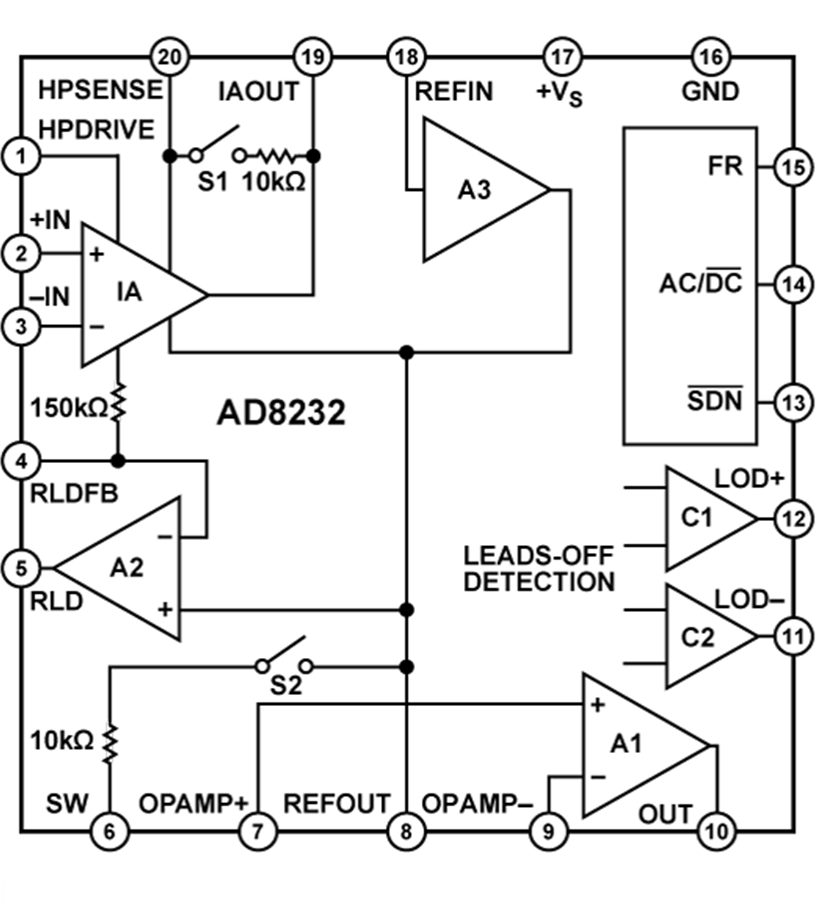
\includegraphics[scale=0.4]{figuras/ecg/ad8232.png}
\caption{Diagrama de bloques funcional}
\label{ad8232}
\end{figure}

Esta figura representa el funcionamiento del integrado y el proceso que realiza en su interior desde el punto de vista de los pines. 
A partir de este diagrama y la herramienta que provee el fabricante para el diseño de filtros, se puede llegar a una configuración del integrado con componentes pasivas para el diseño del circuito impreso como se muestra en la figura \ref{ecgdesign}.\\

\begin{figure}[H]
\centering
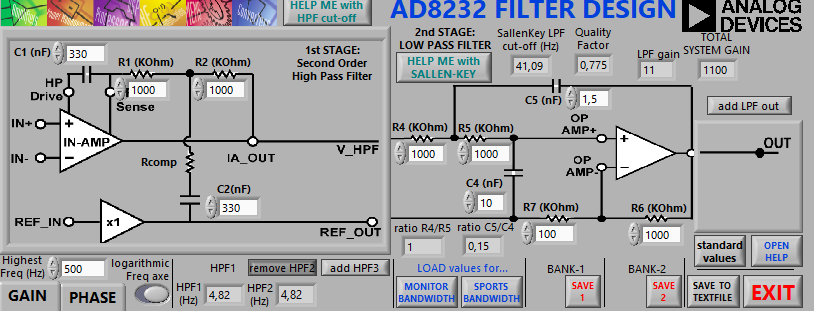
\includegraphics[scale=0.6]{figuras/ecg/ecgdesign.png}
\caption{Herramienta para diseño de filtros}
\label{ecgdesign}
\end{figure}

Como se puede observar en la figura \ref{ecgdesign}, en el lado izquierdo se diseña un filtro pasa alto de segundo orden cuya frecuencia de corte es de 4.82[Hz]. A la derecha se muestra un filtro pasabajo sallen-key con frecuencia de corte 41.09[Hz] donde finalmente se tiene una salida hacia el Arduino. 
Estos valores se obtuvieron al ver el circuito de la PCB de DFRobot (Figura \ref{esquematico11}) y utilizando la herramienta de diseño de filtros. En caso de que se quisieran cambiar las frecuencias de corte se podría hacer un nuevo diseño utilizando el mismo programa pero cambiando y apuntando a frecuencias de corte entre 1-35[Hz] dadas por el dispositivo Biopac.

\begin{figure}[H]
\centering
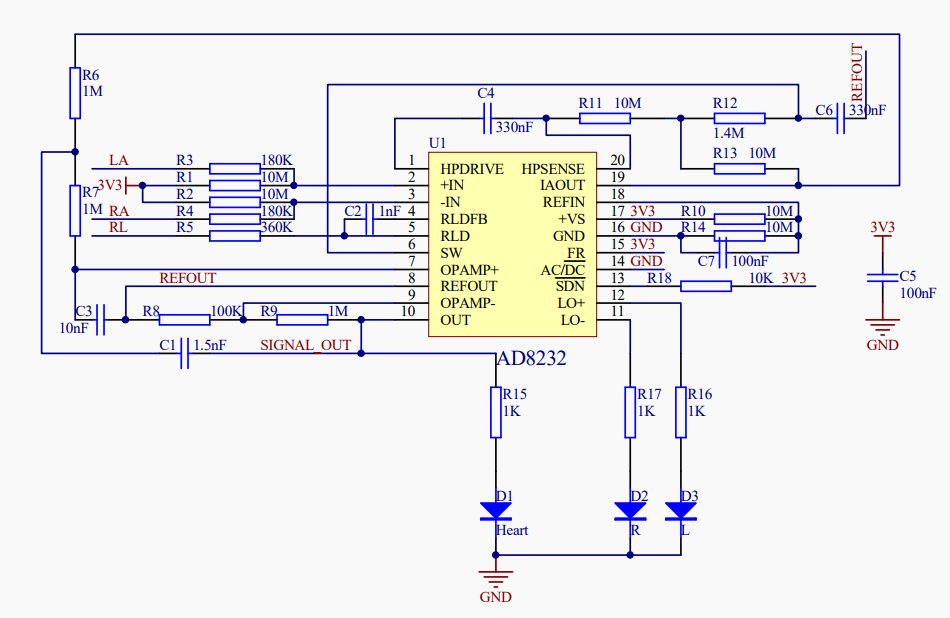
\includegraphics[scale=0.45]{figuras/ecg/esquematico.png}
\caption{Esquemático ECG DFRobot}
\label{esquematico11}
\end{figure}

\newpage
\section{Comparación entre Biopac y DFRobot}
Finalmente se pudo contrastar ambas señales, se puede observar en la figura \ref{graficos} la señal de ECG del Biopac y DFRobot colocando los electrodos muy cerca para obtener las señales lo más parecidas posibles y poder compararlas. 

\begin{figure}[H]
\centering
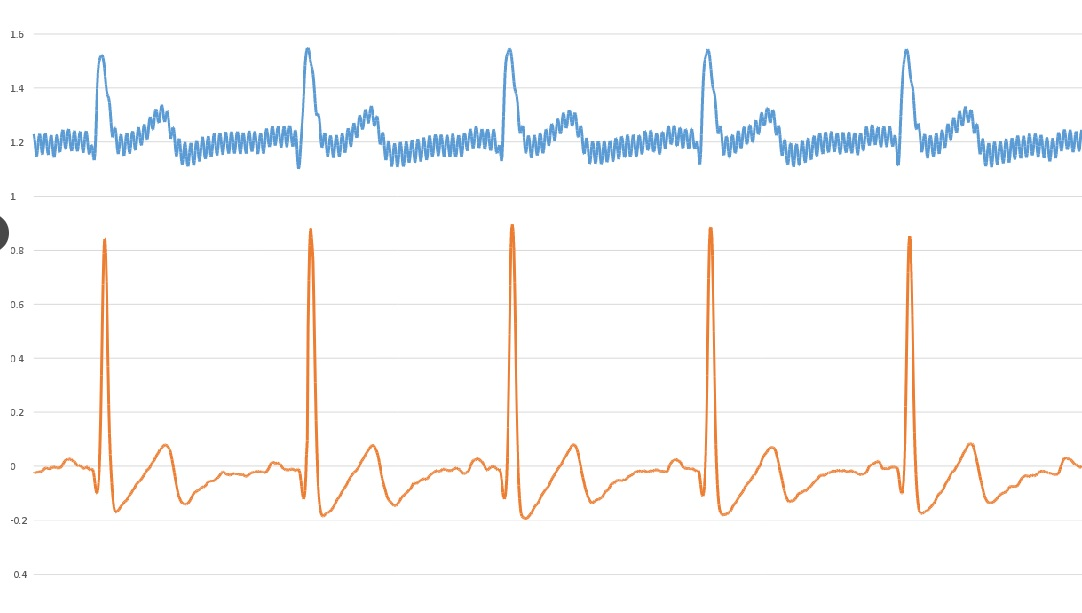
\includegraphics[scale=0.45]{figuras/ecg/biovsdf.jpg}
\caption{Gráfico Biopac ECG100C vs ECG DFRobot}
\label{graficos}
\end{figure}

En el gráfico superior se puede observar la forma de onda del ECG AD8232 en la cual se puede observar notoriamente un ruido de la fuente. En el gráfico inferior se muestra la señal del ECG100C de Biopac, la cual es una señal muy definida a lo cual debería apuntar el diseño del ECG.
Se puede concluir de estas imágenes que la forma de onda de ambas señales son parecidas, considerando que el Biopac está diseñado para mostrar la onda completa, en cambio el AD8232 se encarga de mostrar la onda PR y QT. 
Finalmente se considera que la forma de onda que se tiene sirve para hacer mediciones eliminando el ruido de la fuente ya que es representativa por los peaks que presenta. 

\section{Eliminando ruido de la fuente}
Observando la señal que se tiene actualmente en el dispositivo mediante bluetooth en la aplicación móvil se obtiene una señal como se observa en la figura \ref{ecgfeo}.

\begin{figure}[H]
\centering
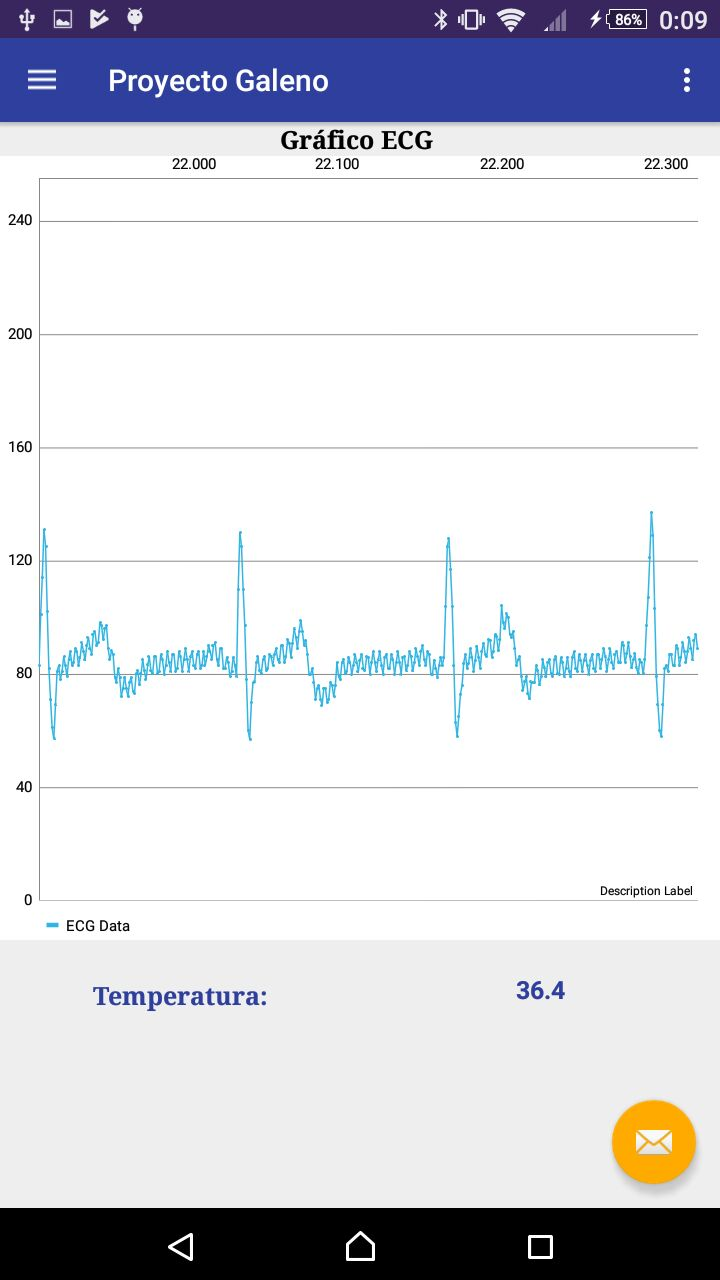
\includegraphics[scale=0.3]{figuras/ecg/ecgappmalo.jpg}
\caption{ECG en aplicación móvil sin filtro de salida}
\label{ecgfeo}
\end{figure}

Se puede notar en esta imagen que la forma de onda se mantiene al enviarla por bluetooth a la aplicación pero sigue con mucho ruido. Utilizando la herramienta de diseño de filtros para el AD8232 existe una opción para filtrar la salida de la señal final, para esto se considera utilizar un filtro pasabajo para eliminar el ruido como se muestra en la figura \ref{filtroout}.

\begin{figure}[H]
\centering
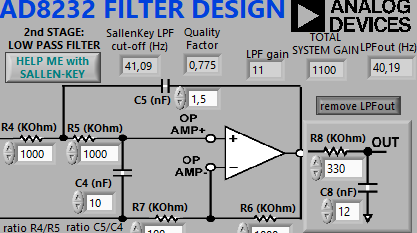
\includegraphics[scale=0.75]{figuras/ecg/filtroout.png}
\caption{Filtgro de salida R8 y C8}
\label{filtroout}
\end{figure}

Se diseñó con frecuencia de corte de $40.19[Hz]$ como se muestra en la figura \ref{filtroout} dando valores $R8 = 330[k\Omega]$ y $C8 = 12[nF]$ para no perder información de la señal y con esto limpiar solamente la señal como se muestra en el resultado de la figura \ref{ecgbonito}

\begin{figure}[H]
\centering
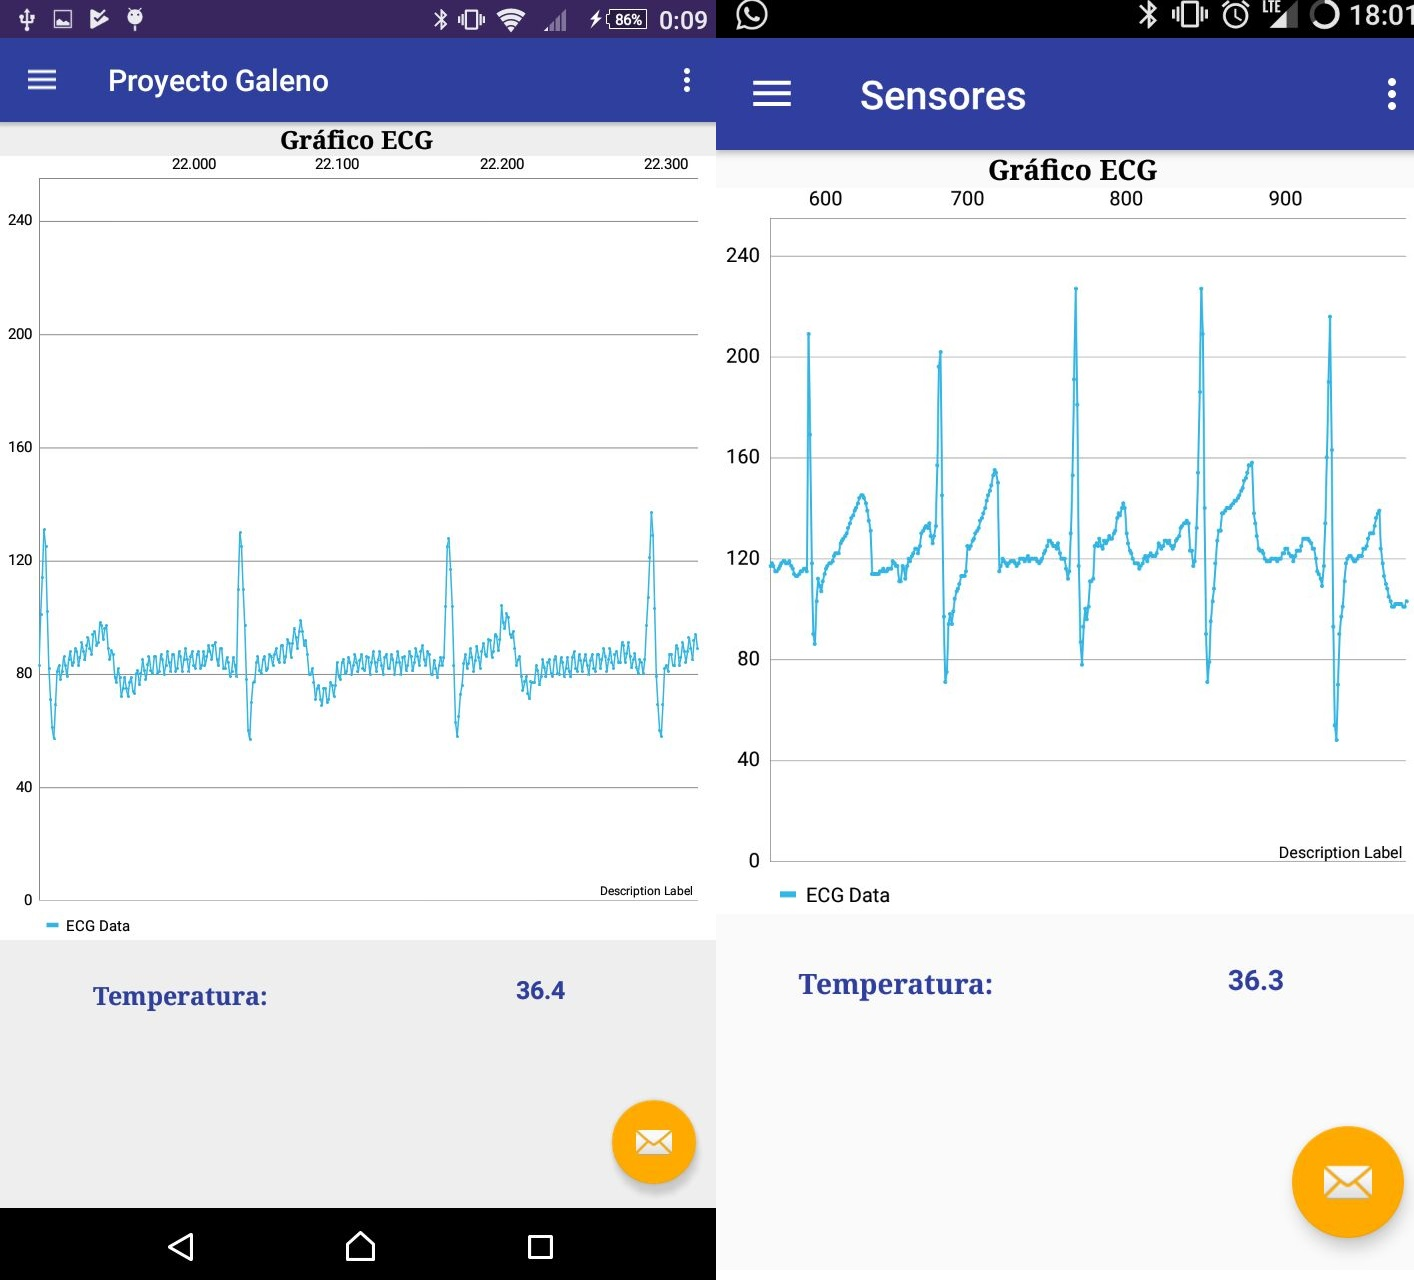
\includegraphics[scale=0.25]{figuras/ecg/ecgappbueno.jpg}
\caption{Comparación ECG en aplicación móvil con filtros de salida}
\label{ecgbonito}
\end{figure}

Se nota un gran cambio en la forma de la señal, donde se notan de mejor manera, sin ruido de la fuente y sin perder la forma de onda. Esta será la configuración que se utilizará para el diseño final del dispositivo.

